\chapter{Metodologia badań}

Niniejszy rozdział poświęcony jest szczegółowemu opisowi aparatu matematycznego oraz metod statystycznych wykorzystanych w procesie analizy empirycznej. Zrozumienie mechanizmów rządzących punktualnością w transporcie lotniczym wymaga wyjścia poza ramy klasycznej ekonometrii liniowej, dlatego fundamentem prowadzonych badań uczyniono modele nieliniowe, które pozwalają na precyzyjne kwantyfikowanie zjawisk o charakterze jakościowym.

\section{Uogólnione Modele Liniowe (GLM) i fundamenty regresji logistycznej}

W modelowaniu zjawisk ekonomicznych, w których zmienna objaśniana przyjmuje wartości dyskretne, standardowe podejście oparte na Klasycznej Metodzie Najmniejszych Kwadratów (KMNK) okazuje się niewystarczające. Modele regresji logistycznej wykorzystywane są powszechnie do objaśniania takich zmiennych jakościowych w zależności od poziomu rozpatrywanych zmiennych egzogenicznych \cite{jackowska2011}. W tym punkcie przedstawione zostaną teoretyczne podstawy przejścia od modeli liniowych do klasy Uogólnionych Modeli Liniowych (GLM), ze szczególnym uwzględnieniem regresji logistycznej.

\subsection{Ograniczenia modelu liniowego (LPM)}

Zastosowanie regresji liniowej do analizy zmiennej jakościowej (np. wystąpienie opóźnienia lub jego brak) prowadzi do powstania Modelu Liniowego Prawdopodobieństwa (ang. \textit{Linear Probability Model} -- LPM). Model ten można zapisać jako:
\begin{equation}
    y_i = \mathbf{x}_i' \boldsymbol{\beta} + \epsilon_i
\end{equation}
gdzie $E(y_i | \mathbf{x}_i) = P(y_i = 1 | \mathbf{x}_i) = \mathbf{x}_i' \boldsymbol{\beta}$. Jak wskazuje W. Greene \cite{greene2003}, takie podejście obarczone jest szeregiem wad, które dyskwalifikują je w profesjonalnych analizach mikroekonometrycznych:

\begin{enumerate}
    \item \textit{Nielogiczne wartości prawdopodobieństwa:} Funkcja liniowa $\mathbf{x}_i' \boldsymbol{\beta}$ nie jest ograniczona w przedziale $[0, 1]$. W praktyce oznacza to, że dla niektórych zestawów zmiennych objaśniających (np. ekstremalne warunki pogodowe), model może oszacować prawdopodobieństwo ujemne lub przekraczające jedność, co jest sprzeczne z aksjomatami Kołmogorowa.
    \item \textit{Heteroskedastyczność:} W modelu LPM wariancja składnika losowego nie jest stała i zależy od wartości zmiennych objaśniających: $Var(\epsilon_i) = \mathbf{x}_i' \boldsymbol{\beta} (1 - \mathbf{x}_i' \boldsymbol{\beta})$. Powoduje to, że estymatory KMNK tracą cechę efektywności, a standardowe błędy oszacowań stają się niewiarygodne \cite{maddala1983}.
    \item \textit{Nienormalność rozkładu składnika losowego:} Ponieważ zmienna $y_i$ przyjmuje tylko dwie wartości, składnik losowy $\epsilon_i$ również musi być dwupunktowy, co uniemożliwia przyjęcie założenia o normalności rozkładu niezbędnego do weryfikacji hipotez statystycznych w małych próbach.
\end{enumerate}

\subsection{Koncepcja Uogólnionych Modeli Liniowych (GLM)}

Problemy modelu LPM rozwiązuje koncepcja GLM, która pozwala na modelowanie wartości oczekiwanej zmiennej zależnej poprzez nieliniową funkcję łączącą. Model logitowy jest w istocie szczególnym przypadkiem uogólnionego modelu liniowego \cite{jackowska2011}. Zgodnie z definicją T. Hastie i in. \cite{hastie2009}, model ten definiują trzy elementy:

\begin{itemize}
    \item \textit{Składnik losowy:} Rozkład zmiennej $y$ należący do rodziny wykładniczej.
    \item \textit{Predyktor liniowy:} $\eta = \beta_0 + \beta_1 x_1 + \dots + \beta_k x_k$.
    \item \textit{Funkcja łącząca (link function):} Funkcja $g(\cdot)$, która wiąże wartość oczekiwaną zmiennej $\mu = E(y)$ z liniową kombinacją predyktorów, zadaną równaniem $g(\mu) = \mathbf{x}' \boldsymbol{\beta}$ \cite{jackowska2011}.
\end{itemize}

\subsection{Regresja logistyczna i pojęcie logitu}

Jeżeli w badaniu zmienna objaśniana przyjmuje dokładnie dwa stany (tzn. informuje nas jednoznacznie, czy badane zjawisko opóźnienia wystąpiło, czy też nie), to mamy do czynienia z modelem dwumianowym \cite{jackowska2011}. W takiej regresji logistycznej funkcją łączącą jest funkcja logitowa. Zakładamy, że prawdopodobieństwo wystąpienia zdarzenia $p$ jest opisane dystrybuantą rozkładu logistycznego:
\begin{equation}
    p_i = \frac{1}{1 + e^{-\mathbf{x}_i' \boldsymbol{\beta}}}
\end{equation}

Kluczowym pojęciem jest tu \textbf{szansa} (ang. \textit{odds}), definiowana jako iloraz prawdopodobieństwa wystąpienia zdarzenia oraz prawdopodobieństwa niewystąpienia tego zdarzenia \cite{jackowska2011}:
\begin{equation}
    \frac{p_i}{1 - p_i} = e^{\mathbf{x}_i' \boldsymbol{\beta}}
\end{equation}

Logarytmując powyższe wyrażenie, otrzymujemy liniową postać modelu, w której wspomniana wcześniej funkcja wiążąca nazywana jest \textbf{logitem} \cite{jackowska2011}:
\begin{equation}
    L_i = \ln \left( \frac{p_i}{1 - p_i} \right) = \beta_0 + \beta_1 x_{i1} + \dots + \beta_k x_{ik}
\end{equation}

Transformacja ta pozwala na estymację parametrów modelu za pomocą metody Największej Wiarygodności (MLE), co w praktyce oznacza maksymalizację logarytmu funkcji wiarygodności przy użyciu numerycznych procedur iteracyjnych \cite{jackowska2011}.

\subsection{Interpretacja parametrów i Ilorazy Szans (Odds Ratios)}

Jedną z największych zalet modelu logitowego jest możliwość stosunkowo prostej interpretacji parametrów $e^{\beta_i}$ \cite{jackowska2011}. Ze względu na logarytmiczną transformację, bezpośrednie współczynniki $\beta$ informują o zmianie logarytmu szansy, a nie samego prawdopodobieństwa. W celu nadania wynikom interpretacji ekonomicznej stosuje się transformację wykładniczą parametrów, wyznaczając tzw. \textbf{Ilorazy Szans} (ang. \textit{Odds Ratios} -- OR):
\begin{equation}
    OR = \exp(\beta_j)
\end{equation}

Interpretacja wyników zależy od charakteru zmiennych oraz przypisanych wartości bazowych:
\begin{itemize}
    \item \textit{Wyraz wolny:} wartość $e^{\beta_0}$ interpretowana jest jako szansa wystąpienia zjawiska w grupie referencyjnej, dla której wszystkie pozostałe zmienne objaśniające wynoszą zero \cite{jackowska2011}.
    \item \textit{Zmienna dychotomiczna:} jeżeli badana zmienna $x_j$ jest zmienną zero-jedynkową, to uzyskany współczynnik $e^{\beta_j}$ jest równy ilorazowi szans dla grupy, w której zmienna przyjmuje wartość 1, w stosunku do grupy, gdzie zmienna równa jest 0, przy zachowaniu stałości pozostałych parametrów \cite{jackowska2011}.
    \item \textit{Zmienna ilościowa:} w przypadku zmiennych ciągłych iloraz szans $e^{\beta_j}$ informuje, jak zmieni się szansa wystąpienia opóźnienia, jeżeli zmienna ta wzrośnie o dokładnie jedną jednostkę \cite{jackowska2011}.
\end{itemize}

Ogólnie wskaźnik $OR$ pozwala na szybką identyfikację kierunku wpływu: $OR > 1$ oznacza, że wzrost zmiennej objaśniającej zwiększa szansę wystąpienia zdarzenia, natomiast $OR < 1$ wskazuje na relację odwrotną. Wartość $OR = 1$ oznacza brak istotnego wpływu zmiennej na szansę wystąpienia badanego zjawiska.

\section{Uporządkowany model wielomianowy (Ordered Logit Model)}

W praktyce analitycznej zjawisk społeczno-gospodarczych często spotyka się sytuacje, w których zmienna objaśniana ma charakter jakościowy, a jej warianty (kategorie) pozostają w ściśle określonej, naturalnej hierarchii. Przykładem takiej struktury są stopnie oceny ryzyka kredytowego, poziomy wykształcenia, czy – jak w przypadku niniejszej pracy – rosnące kategorie wielkości opóźnień w transporcie lotniczym. W takich przypadkach aparat analityczny musi zostać odpowiednio rozszerzony, a właściwym narzędziem statystycznym staje się uporządkowany model wielomianowy (ang. \textit{Ordered Logit Model} lub \textit{Proportional Odds Model}).

\subsection{Rozszerzenie modelu binarnego na dane porządkowe}

Klasyczna regresja logistyczna, ze względu na swoją architekturę, ogranicza się do modelowania zjawisk dychotomicznych (dwustanowych). Próba analizy zjawisk wieloklasowych za pomocą prostych modeli napotyka na fundamentalne przeszkody. Jak zauważa G.S. Maddala \cite{maddala1983}, zastosowanie zwykłej Klasycznej Metody Najmniejszych Kwadratów (KMNK) do danych porządkowych poprzez przypisanie im arbitralnych wartości liczbowych (np. 1 dla małego opóźnienia, 2 dla średniego, 3 dla dużego) jest błędem metodologicznym. Regresja liniowa zakłada bowiem, że dystans (różnica natężenia cechy) między kategorią 1 a 2 jest dokładnie taki sam, jak między kategorią 2 a 3. W rzeczywistości rynkowej odstępy te są nieznane i z reguły asymetryczne. 

Alternatywą mogłoby być zastosowanie nieuporządkowanego modelu wielomianowego (ang. \textit{Multinomial Logit Model}), który rozszerza analizę na wiele klas. Jednakże model ten traktuje kategorie jako całkowicie niezależne i nominalne (jak np. wybór środka transportu: pociąg, autobus, samolot). Zastosowanie go do danych o opóźnieniach prowadziłoby do bezpowrotnej utraty cennej informacji o tym, że opóźnienie średnie jest w naturalny sposób "gorsze" od małego, a mniejsze od krytycznego. Uporządkowany model logitowy rozwiązuje ten problem, stanowiąc ewolucyjne rozwinięcie modelu binarnego, w którym mechanizm szacowania prawdopodobieństw uwzględnia i chroni porządkowy charakter (ranking) analizowanych klas \cite{greene2003}.

\subsection{Koncepcja zmiennej ukrytej (Latent Variable)}

Fundamentem teoretycznym uporządkowanego modelu wielomianowego jest założenie o istnieniu w systemie nieobserwowalnej, ciągłej zmiennej ukrytej, oznaczanej w literaturze ekonometrycznej jako $y^*$. Zmienną tę należy interpretować jako niemierzalną bezpośrednio "skłonność" (ang. \textit{propensity}) badanego systemu do wygenerowania określonego zdarzenia – w tym wypadku: skłonność systemu operacyjnego linii lotniczej do generowania zakłóceń czasowych \cite{greene2003}. 

Zmienna ukryta opisana jest ciągłym równaniem strukturalnym, które w zapisie macierzowym przyjmuje postać:
\begin{equation}
    y_i^* = \mathbf{x}_i' \boldsymbol{\beta} + \varepsilon_i \quad \text{dla} \quad i = 1, \dots, n
\end{equation}
gdzie:
\begin{itemize}
    \item $y_i^*$ oznacza wartość ciągłej, nieobserwowalnej zmiennej ukrytej dla $i$-tej obserwacji;
    \item $\mathbf{x}_i$ jest wektorem wartości zmiennych objaśniających (predyktorów), takich jak warunki meteorologiczne, infrastrukturalne czy organizacyjne;
    \item $\boldsymbol{\beta}$ to wektor nieznanych parametrów strukturalnych (współczynników modelu), które odzwierciedlają kierunek i siłę wpływu poszczególnych zmiennych na skłonność do opóźnień;
    \item $\varepsilon_i$ reprezentuje losowy składnik błędu (składnik resztowy).
\end{itemize}

Kluczowym założeniem modelu logitowego jest przyjęcie specyficznego rozkładu dla składnika losowego $\varepsilon_i$. Zakłada się, że posiada on standardowy rozkład logistyczny o wartości oczekiwanej równej zero ($E(\varepsilon) = 0$) oraz wariancji równej $\pi^2/3$. Dystrybuanta tego rozkładu, oznaczana najczęściej jako $\Lambda(\cdot)$ lub $F(\cdot)$, wyraża się zwartym wzorem analitycznym:
\begin{equation}
    F(\varepsilon) = \frac{\exp(\varepsilon)}{1 + \exp(\varepsilon)}
\end{equation}
To właśnie właściwości tego rozkładu – w szczególności nieznacznie "grubsze ogony" w porównaniu z rozkładem normalnym – sprawiają, że modele logitowe charakteryzują się wysoką odpornością (ang. \textit{robustness}) na występowanie w próbie badawczej wartości odstających, co jest zjawiskiem niezwykle powszechnym w masowych danych transportowych \cite{hastie2009}.



\subsection{Mechanika progów (Cut-points) i prawdopodobieństwa warunkowe}

Chociaż zmienna ukryta $y^*$ ma charakter ciągły i rozciąga się od minus do plus nieskończoności, w rzeczywistości badacz obserwuje jedynie dyskretne, kategoryczne realizacje tej zmiennej, oznaczane jako $y$. Związek pomiędzy nieobserwowalną skłonnością $y_i^*$ a empirycznie obserwowalną kategorią $y_i$ definiuje mechanizm progów odcięcia (ang. \textit{cut-points} lub \textit{thresholds}), oznaczanych grecką literą $\mu$.

W modelu uwzględniającym $J$ uporządkowanych kategorii istnieje dokładnie $J-1$ nieznanych progów odcięcia. Proces dyskretyzacji zmiennej ukrytej przebiega według następującego schematu \cite{greene2003}:
\begin{equation}
    y_i = \begin{cases} 
    1 & \text{jeżeli } y_i^* \le \mu_1 \\
    2 & \text{jeżeli } \mu_1 < y_i^* \le \mu_2 \\
    3 & \text{jeżeli } \mu_2 < y_i^* \le \mu_3 \\
    \vdots & \vdots \\
    J & \text{jeżeli } y_i^* > \mu_{J-1}
    \end{cases}
\end{equation}

Aby model był możliwy do oszacowania (identyfikowalny matematycznie), musi zostać spełniony warunek ścisłej monotoniczności progów: $\mu_1 < \mu_2 < \dots < \mu_{J-1}$. Progi te pełnią funkcję "barier przejścia". W kontekście lotniczym, wraz z pogarszaniem się warunków (np. wzrostem siły wiatru), rośnie wartość zmiennej ukrytej $y^*$. Kiedy $y^*$ przekracza pierwszy próg $\mu_1$, opóźnienie lotu przeskakuje z kategorii małej do średniej. Przekroczenie kolejnego progu $\mu_2$ oznacza już kategoryzację zdarzenia jako opóźnienia wielkiego (krytycznego).

Ponieważ równanie strukturalne zawiera składnik losowy $\varepsilon_i$, nie można ze stuprocentową pewnością określić, do której kategorii trafi dana obserwacja. Zamiast tego, ekonometria pozwala na wyliczenie prawdopodobieństwa warunkowego, z jakim obserwacja znajdzie się w określonej klasie, pod warunkiem zaobserwowania danego wektora $\mathbf{x}_i$. 

Prawdopodobieństwo, że zmienna obserwowana $y$ przyjmie wartość równą lub mniejszą od $j$, jest równoznaczne z prawdopodobieństwem, że zmienna ukryta $y^*$ nie przekroczy progu $\mu_j$. Wykorzystując dystrybuantę rozkładu logistycznego $F(\cdot)$, można zapisać to prawdopodobieństwo skumulowane następująco \cite{maddala1983}:
\begin{equation}
    P(y_i \le j | \mathbf{x}_i) = P(y_i^* \le \mu_j) = P(\mathbf{x}_i' \boldsymbol{\beta} + \varepsilon_i \le \mu_j) = P(\varepsilon_i \le \mu_j - \mathbf{x}_i' \boldsymbol{\beta})
\end{equation}
Co po podstawieniu do wzoru na dystrybuantę daje ostateczną postać modelu prawdopodobieństwa skumulowanego:
\begin{equation}
    P(y_i \le j | \mathbf{x}_i) = \frac{1}{1 + \exp(-(\mu_j - \mathbf{x}_i' \boldsymbol{\beta}))}
\end{equation}

Ostatecznie, aby obliczyć prawdopodobieństwo przynależności badanej jednostki do jednej, konkretnej kategorii $j$, należy wyznaczyć różnicę odpowiednich wartości dystrybuanty. Geometria tego zagadnienia sprowadza się do obliczenia pola pod krzywą rozkładu logistycznego, znajdującego się pomiędzy dwoma sąsiadującymi progami odcięcia:
\begin{equation}
    P(y_i = j | \mathbf{x}_i) = F(\mu_j - \mathbf{x}_i' \boldsymbol{\beta}) - F(\mu_{j-1} - \mathbf{x}_i' \boldsymbol{\beta})
\end{equation}

Dla skrajnych przedziałów przyjmuje się, że $\mu_0 = -\infty$ oraz $\mu_J = +\infty$, co sprawia, że dystrybuanta $F(-\infty) = 0$, a $F(+\infty) = 1$. Zatem dla pierwszej kategorii ($j=1$) wzór upraszcza się do $F(\mu_1 - \mathbf{x}_i' \boldsymbol{\beta})$, a dla kategorii ostatniej ($j=J$) do $1 - F(\mu_{J-1} - \mathbf{x}_i' \boldsymbol{\beta})$.

\begin{figure}[htbp]
    \centering
    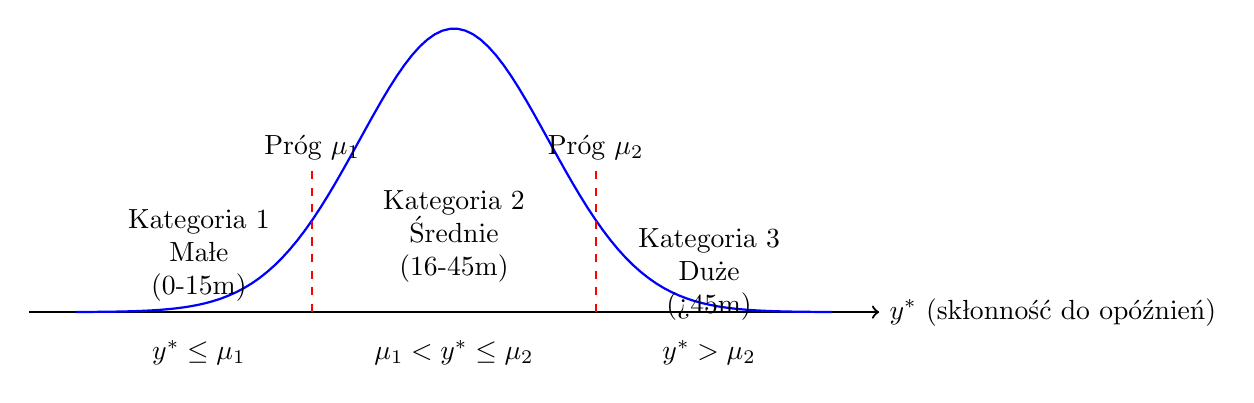
\begin{tikzpicture}[scale=1.2]
        % Oś X (Zmienna ukryta y*)
        \draw[->, thick] (-4,0) -- (5,0) node[right] {$y^*$ (skłonność do opóźnień)};
        
        % Krzywa rozkładu (przybliżenie rozkładu logistycznego/normalnego)
        \draw[thick, blue] plot[domain=-3.5:4.5, samples=100] (\x, {3*exp(-(\x-0.5)^2/2)});
        
        % Progi odcięcia (Cut-points)
        \draw[dashed, thick, red] (-1, 0) -- (-1, 1.5) node[above, text=black] {Próg $\mu_1$};
        \draw[dashed, thick, red] (2, 0) -- (2, 1.5) node[above, text=black] {Próg $\mu_2$};
        
        % Oznaczenia obszarów (Kategorie opóźnień)
        \node[align=center] at (-2.2, 0.6) {Kategoria 1\\ Małe \\ (0-15m)};
        \node[align=center] at (0.5, 0.8) {Kategoria 2\\ Średnie \\ (16-45m)};
        \node[align=center] at (3.2, 0.4) {Kategoria 3\\ Duże \\ (>45m)};
        
        % Etykiety prawdopodobieństw pod osią X
        \node[below] at (-2.2, -0.2) {$y^* \le \mu_1$};
        \node[below] at (0.5, -0.2) {$\mu_1 < y^* \le \mu_2$};
        \node[below] at (3.2, -0.2) {$y^* > \mu_2$};
    \end{tikzpicture}
    \caption{Mechanika progów odcięcia i kategoryzacja zmiennej ukrytej w modelu Ordered Logit.}
    \label{fig:ordered_logit_plot}
\end{figure}

\subsection{Założenie o proporcjonalności szans (Parallel Regression Assumption)}

Należy podkreślić, że klasyczny Uporządkowany Model Logitowy opiera się na bardzo restrykcyjnym założeniu, znanym jako założenie o proporcjonalności szans (ang. \textit{Proportional Odds Assumption} lub \textit{Parallel Regression Assumption}). Oznacza to, że wektor parametrów strukturalnych $\boldsymbol{\beta}$ jest identyczny i stały (niezmienniczy) dla wszystkich punktów podziału $j$ \cite{greene2003}.

W ujęciu algebraicznym, model zakłada, że krzywe prawdopodobieństwa opisujące poszczególne kategorie są względem siebie idealnie równoległe, a to, co ulega zmianie przy przejściu między kategoriami, to wyłącznie współczynniki wyrazu wolnego, reprezentowane przez wartości progów odcięcia $\mu_j$ \cite{jackowska2011}. Oznacza to, że wpływ danej zmiennej objaśniającej (np. spadku temperatury) na szansę przesunięcia się lotu z kategorii punktualnej do opóźnionej jest strukturalnie dokładnie taki sam, jak wpływ tej samej zmiennej na przesunięcie się lotu z opóźnienia małego do kategorii ekstremalnego, wielogodzinnego zatoru. Właściwość ta nadaje modelowi ogromną elegancję matematyczną i stabilność estymatorów, a oszacowane parametry zachowują globalny, uniwersalny charakter w odniesieniu do całego spektrum analizowanego zjawiska. 

\section{Estymacja parametrów modelu metodą Największej Wiarygodności}

Wybór odpowiedniej metody szacowania parametrów strukturalnych jest determinowany przez nieliniowy charakter funkcji prawdopodobieństwa w modelu \textit{Ordered Logit}. W przeciwieństwie do modeli liniowych, gdzie dominującym narzędziem jest Klasyczna Metoda Najmniejszych Kwadratów, w modelach zmiennych jakościowych standardem jest metoda Największej Wiarygodności (ang. \textit{Maximum Likelihood Estimation} -- MLE).

\subsection{Zasada działania i fundamenty koncepcyjne MLE}

Istota metody Największej Wiarygodności opiera się na odwróceniu perspektywy klasycznego wnioskowania probabilistycznego. O ile rachunek prawdopodobieństwa pozwala określić szansę wystąpienia danych przy znanych parametrach populacji, o tyle MLE służy do znalezienia takich wartości parametrów $\boldsymbol{\beta}$ oraz $\boldsymbol{\mu}$, dla których zaobserwowana w próbie badawczej kombinacja zdarzeń jest najbardziej prawdopodobna \cite{greene2003}. 

Koncepcyjnie metoda ta zakłada, że posiadana próba danych jest reprezentatywnym odzwierciedleniem procesu generującego dane. Szukamy zatem wektora parametrów, który maksymalizuje funkcję wiarygodności, co w ujęciu statystycznym zapewnia uzyskanie estymatorów o pożądanych właściwościach asymptotycznych: zgodności, asymptycznej efektywności oraz asymptycznej normalności \cite{diebold1996}. Jak wskazują Diebold i Schuermann \cite{diebold1996}, precyzyjne (dokładne) podejście do konstrukcji funkcji wiarygodności jest kluczowe dla zachowania jakości predykcji w modelach ekonometrycznych operujących na dużych zbiorach danych.

\subsection{Konstrukcja funkcji wiarygodności i log-wiarygodności}

Punktem wyjścia do estymacji jest zdefiniowanie funkcji wiarygodności $L(\boldsymbol{\beta}, \boldsymbol{\mu})$, która dla niezależnych obserwacji jest iloczynem prawdopodobieństw wystąpienia konkretnych kategorii $j$, zaobserwowanych dla każdej $i$-tej jednostki w próbie. Można ją zapisać jako:
\begin{equation}
    L(\boldsymbol{\beta}, \boldsymbol{\mu}) = \prod_{i=1}^{n} \prod_{j=1}^{J} [P(y_i = j | \mathbf{x}_i)]^{d_{ij}}
\end{equation}
gdzie $d_{ij}$ jest zmienną indykatorową przyjmującą wartość 1, jeżeli dla $i$-tej obserwacji wystąpiła kategoria $j$, oraz 0 w przeciwnym razie. Podstawiając wyprowadzone wcześniej wzory na prawdopodobieństwa w modelu \textit{Ordered Logit}, otrzymujemy:
\begin{equation}
    L(\boldsymbol{\beta}, \boldsymbol{\mu}) = \prod_{i=1}^{n} \prod_{j=1}^{J} [F(\mu_j - \mathbf{x}_i' \boldsymbol{\beta}) - F(\mu_{j-1} - \mathbf{x}_i' \boldsymbol{\beta})]^{d_{ij}}
\end{equation}

Z operacyjnego punktu widzenia, maksymalizacja iloczynu wielu prawdopodobieństw jest zadaniem trudnym numerycznie. Dlatego w praktyce ekonometrycznej dokonuje się transformacji logarytmicznej, przechodząc do logarytmicznej funkcji wiarygodności (ang. \textit{Log-Likelihood}):
\begin{equation}
    \ln L(\boldsymbol{\beta}, \boldsymbol{\mu}) = \sum_{i=1}^{n} \sum_{j=1}^{J} d_{ij} \ln [F(\mu_j - \mathbf{x}_i' \boldsymbol{\beta}) - F(\mu_{j-1} - \mathbf{x}_i' \boldsymbol{\beta})]
\end{equation}

Transformacja ta jest dopuszczalna, ponieważ funkcja logarytmiczna jest monotonicznie rosnąca, co oznacza, że maksimum funkcji $L$ oraz $\ln L$ przypada dla tych samych wartości parametrów. Postać addytywna (suma zamiast iloczynu) znacząco ułatwia obliczanie pochodnych cząstkowych niezbędnych do wyznaczenia warunków pierwszego rzędu.



\subsection{Procedury iteracyjne i optymalizacja numeryczna}

W przypadku modelu \textit{Ordered Logit} warunki konieczne istnienia ekstremum (\textit{First Order Conditions}) prowadzą do układu równań nieliniowych względem parametrów $\boldsymbol{\beta}$ oraz $\boldsymbol{\mu}$. W przeciwieństwie do regresji liniowej, nie istnieje tutaj rozwiązanie w postaci jawnego wzoru analitycznego (\textit{closed-form solution}) \cite{maddala1983}.

W związku z powyższym, szacowanie parametrów odbywa się przy użyciu numerycznych algorytmów iteracyjnych. Najczęściej wykorzystywaną metodą jest algorytm Newtona-Raphsona lub jego modyfikacje (np. metoda BFGS). Proces ten przebiega w kilku etapach:
\begin{enumerate}
    \item \textit{Inicjalizacja:} Przyjęcie początkowych wartości parametrów (często na podstawie uproszczonych modeli liniowych).
    \item \textit{Gradient i Hesjan:} Wyznaczenie wektora pochodnych cząstkowych (gradientu) oraz macierzy drugich pochodnych (macierzy informacyjnej/Hesjanu), która wskazuje kierunek i "stromość" wzrostu funkcji wiarygodności.
    \item \textit{Aktualizacja:} Korygowanie wartości parametrów w kierunku maksimum aż do momentu, gdy przyrost funkcji wiarygodności stanie się pomijalnie mały (osiągnięcie zbieżności).
\end{enumerate}

Poprawność procesu estymacji w dużej mierze zależy od globalnej wklęsłości funkcji log-wiarygodności. Jak wskazuje J.M. Wooldridge, dla rozkładu logistycznego funkcja ta jest zazwyczaj dobrze uwarunkowana, co gwarantuje zbieżność algorytmów do globalnego maksimum, zapewniając stabilność uzyskanych wyników empirycznych \cite{jackowska2011}. Osiągnięte w ten sposób oszacowania stanowią podstawę do dalszej interpretacji efektów krańcowych oraz weryfikacji istotności statystycznej badanych uwarunkowań opóźnień lotniczych.

\section{Weryfikacja założeń i diagnostyka modelu}

Proces budowy modelu ekonometrycznego nie kończy się na estymacji jego parametrów. Aby uzyskane wyniki mogły służyć do rzetelnego wnioskowania o przyczynach opóźnień lotniczych, konieczna jest rygorystyczna weryfikacja założeń statystycznych oraz ocena dobroci dopasowania modelu do danych empirycznych. W przypadku uporządkowanego modelu logitowego kluczowym punktem diagnostycznym jest sprawdzenie stabilności parametrów strukturalnych oraz weryfikacja siły predykcyjnej klasyfikatora.

\subsection{Założenie o proporcjonalności szans (Parallel Regression Assumption)}

Najbardziej krytycznym założeniem modelu \textit{Ordered Logit} jest założenie o proporcjonalności szans, znane również jako założenie o równoległości regresji (\textit{Parallel Regression Assumption}). Jak wskazuje W. Greene \cite{greene2003}, model ten zakłada, że wektor parametrów $\boldsymbol{\beta}$ pozostaje stały niezależnie od tego, przez który punkt odcięcia (próg $\mu_j$) dokonujemy podziału zmiennej ukrytej. 

Matematycznie oznacza to, że wpływ zmiennych objaśniających na logarytm szansy skumulowanej jest identyczny dla wszystkich kategorii:
\begin{equation}
    \ln\left( \frac{P(y_i \le j | \mathbf{x}_i)}{1 - P(y_i \le j | \mathbf{x}_i)} \right) = \mu_j - \mathbf{x}_i' \boldsymbol{\beta}
\end{equation}
W powyższym równaniu indeks $j$ występuje przy progu $\mu$, ale nie przy wektorze $\boldsymbol{\beta}$. Oznacza to, że krzywe prawdopodobieństwa skumulowanego dla poszczególnych kategorii są względem siebie równoległe, a zmienia się jedynie ich przesunięcie określane przez progi $\mu$. 

Weryfikacja tego założenia, najczęściej przeprowadzana za pomocą \textit{testu Branta} lub testu ilorazu wiarygodności, jest niezbędna. Jego naruszenie sugeruje, że dana zmienna objaśniająca (np. siła wiatru lub specyfika linii lotniczej) może mieć zupełnie inny wpływ na prawdopodobieństwo wystąpienia małego opóźnienia, a inny na prawdopodobieństwo wystąpienia opóźnienia krytycznego. W sytuacji odrzucenia tego założenia, konieczne byłoby zastosowanie bardziej złożonych modeli, takich jak nieuporządkowany model wielomianowy (\textit{Multinomial Logit}) lub uogólniony uporządkowany model logitowy (\textit{Generalized Ordered Logit}), co jednak wiąże się ze znacznym wzrostem liczby parametrów i utratą przejrzystości interpretacyjnej \cite{maddala1983}.

\subsection{Kryteria informacyjne i miary dopasowania modelu}

W ekonometrii modeli zmiennych jakościowych, gdzie nie jest możliwe zastosowanie klasycznego współczynnika determinacji $R^2$ znanego z metody KMNK, do oceny jakości modelu wykorzystuje się miary oparte na wartości funkcji wiarygodności.

\textit{Kryterium Informacyjne Akaike (AIC)}
Kryterium AIC jest jednym z najpowszechniej stosowanych narzędzi do porównywania modeli o różnej liczbie zmiennych objaśniających. Jego wzór przyjmuje postać:
\begin{equation}
    AIC = 2k - 2\ln(L)
\end{equation}
gdzie $k$ oznacza liczbę parametrów w modelu, a $\ln(L)$ jest wartością zlogarytmowanej funkcji wiarygodności w punkcie optimum. Kluczową cechą AIC jest wprowadzenie kary za nadmierne rozbudowywanie modelu ($2k$). Pozwala to uniknąć zjawiska przeuczenia (\textit{overfitting}), promując modele, które osiągają wysoką wiarygodność przy zachowaniu oszczędności strukturalnej. Przy porównywaniu zestawu modeli, za najlepszy uznaje się ten, który charakteryzuje się najniższą wartością wskaźnika AIC \cite{greene2003}.

\textit{Pseudo R-kwadrat McFaddena}
Inną ważną miarą diagnostyczną jest współczynnik \textit{Pseudo $R^2$}, wśród których najczęściej raportowany jest wskaźnik zaproponowany przez D. McFaddena. Informuje on o tym, o ile lepszy jest model z predyktorami w porównaniu do modelu bazowego (zawierającego jedynie progi odcięcia). Oblicza się go według wzoru:
\begin{equation}
    R^2_{McFadden} = 1 - \frac{\ln(L_{full})}{\ln(L_{null})}
\end{equation}
gdzie $L_{full}$ to wiarygodność modelu pełnego, a $L_{null}$ to wiarygodność modelu bez zmiennych objaśniających. Należy pamiętać, że w modelach logitowych wartości rzędu 0,2--0,4 są już uznawane za dowód bardzo dobrego dopasowania modelu do danych \cite{maddala1983}, co stanowi istotną różnicę w porównaniu do interpretacji $R^2$ w regresji liniowej.

\subsection{Ewaluacja klasyfikacyjna i znaczenie metryk jakości}

Współczesne podejście do diagnostyki modeli, silnie wspierane przez literaturę z zakresu uczenia maszynowego, kładzie duży nacisk na zdolność predykcyjną modelu. AlBassam i AlShahrani \cite{albassam2025} podkreślają, że w przypadku analizy opóźnień lotniczych – gdzie klasy są często niezbalansowane – same miary oparte na wiarygodności mogą być niewystarczające.

W związku z tym, uzupełnieniem diagnostyki ekonometrycznej jest analiza macierzy pomyłek oraz wyznaczenie wskaźników takich jak czułość (\textit{recall}) i precyzja (\textit{precision}). Pozwalają one ocenić, jak skutecznie model \textit{Ordered Logit} radzi sobie z identyfikacją konkretnych kategorii opóźnień. Triangulacja miar ekonometrycznych (AIC, Pseudo $R^2$) z miarami klasyfikacyjnymi zapewnia kompleksową ocenę rzetelności przeprowadzonego badania i pozwala na uniknięcie błędnych wniosków wynikających z asymetrii zbioru danych \cite{albassam2025, jackowska2011}.

\section{Metryki predykcyjne i ocena jakości klasyfikatorów}

Ostatnim etapem budowy fundamentu metodologicznego jest zdefiniowanie narzędzi pozwalających na ocenę zdolności predykcyjnej modelu. O ile miary oparte na wiarygodności (jak AIC czy Pseudo $R^2$) informują o dopasowaniu statystycznym, o tyle metryki klasyfikacyjne pozwalają ocenić realną użyteczność modelu w przewidywaniu konkretnych stanów opóźnień. W obliczu masowego charakteru danych lotniczych, ocena ta musi uwzględniać fakt, iż poszczególne kategorie opóźnień występują z różną częstotliwością \cite{albassam2025}.

\subsection{Wieloklasowa macierz pomyłek (Confusion Matrix)}

Podstawowym narzędziem diagnostycznym w procesie ewaluacji klasyfikatorów jest macierz pomyłek. Jest to zestawienie w formie tabelarycznej, które konfrontuje rzeczywiste przynależności obserwacji do poszczególnych klas z wynikami przewidywanymi przez model. Dla problemu o $J$ kategoriach, macierz ta przyjmuje postać kwadratową o wymiarach $J \times J$. 

Teoretyczne rozpisanie macierzy opiera się na czterech podstawowych komponentach, definiowanych w ujęciu „jeden kontra reszta” (\textit{one-vs-all}) dla każdej kategorii $j$:
\begin{itemize}
    \item \textit{True Positive (TP):} liczba przypadków, w których model poprawnie przewidział kategorię $j$ (np. model trafnie wskazał duże opóźnienie).
    \item \textit{True Negative (TN):} liczba przypadków, w których model poprawnie wykluczył przynależność do kategorii $j$.
    \item \textit{False Positive (FP):} błąd pierwszego rodzaju; sytuacja, w której model błędnie przypisał obserwację do kategorii $j$, choć w rzeczywistości należała ona do innej klasy.
    \item \textit{False Negative (FN):} błąd drugiego rodzaju; sytuacja, w której model pominął obserwację faktycznie należącą do kategorii $j$.
\end{itemize}

Jak wskazują Hastie i in. \cite{hastie2009}, analiza macierzy pomyłek pozwala na identyfikację konkretnych słabości modelu – na przykład tendencji do mylenia opóźnień średnich z dużymi, co jest kluczowe z punktu widzenia operacyjnego zarządzania ruchem lotniczym.

\subsection{Wskaźniki jakości klasyfikacji}

Na podstawie składowych macierzy pomyłek wyprowadza się zestaw wskaźników pozwalających na ilościową ocenę jakości predykcji. Najbardziej intuicyjną miarą jest ogólna trafność modelu (\textit{Accuracy}), definiowana jako stosunek poprawnych diagnoz do wszystkich obserwacji:
\begin{equation}
    Accuracy = \frac{\sum_{j=1}^{J} TP_j}{N}
\end{equation}
gdzie $N$ oznacza całkowitą liczebność próby. Należy jednak zaznaczyć, że miara ta bywa myląca w przypadku zbiorów asymetrycznych. Jeśli 80\% lotów w próbie jest punktualnych, model ignorujący opóźnienia i zawsze przewidujący punktualność osiągnie pozornie wysoką trafność 80\%, będąc jednocześnie bezużytecznym w prognozowaniu zakłóceń \cite{albassam2025}.

Z tego względu konieczne jest wprowadzenie dwóch uzupełniających metryk:
\begin{enumerate}
    \item \textit{Precyzja (Precision):} odsetek poprawnych przewidzeń danej klasy wśród wszystkich przypadków, które model zaklasyfikował do tej klasy. Odpowiada na pytanie: jak dużą pewność mamy, że gdy model przewiduje duże opóźnienie, to ono faktycznie wystąpi?
    \begin{equation}
        Precision = \frac{TP}{TP + FP}
    \end{equation}
    \item \textit{Czułość (Recall / Sensitivity):} zdolność modelu do wykrywania wszystkich przypadków należących do danej klasy. Odpowiada na pytanie: jaki odsetek faktycznych dużych opóźnień został wykryty przez model?
    \begin{equation}
        Recall = \frac{TP}{TP + FN}
    \end{equation}
\end{enumerate}

\subsection{F1-Score jako optymalna miara dla zbiorów niezbalansowanych}

W analizie opóźnień lotniczych badacz staje przed dylematem wyboru między wysoką precyzją a wysoką czułością. Rozwiązaniem tego problemu jest wskaźnik \textit{F1-Score}, stanowiący średnią harmoniczną obu tych miar:
\begin{equation}
    F1 = 2 \cdot \frac{Precision \cdot Recall}{Precision + Recall}
\end{equation}

Zastosowanie średniej harmonicznej zamiast arytmetycznej powoduje, że \textit{F1-Score} karze skrajnie niskie wartości jednego z komponentów. Model, który ma doskonałą czułość, ale fatalną precyzję, otrzyma niską notę końcową. 

Współczesna literatura \cite{albassam2025, hastie2009} uznaje \textit{F1-Score} za optymalną metrykę w badaniach, gdzie występuje tzw. gruby ogon rozkładu lub znaczna dysproporcja klas. W badaniu punktualności lotów, gdzie priorytetem jest wykrywanie rzadszych, ale kosztownych „dużych opóźnień”, \textit{F1-Score} pozwala na rzetelną ocenę, czy model rzeczywiście uczy się wzorców opóźnień, czy jedynie adaptuje się do dominującej klasy lotów punktualnych.

\section*{Przejście do części empirycznej}
\addcontentsline{toc}{section}{Przejście do części empirycznej}

Zarysowany w niniejszym rozdziale aparat metodologiczny – obejmujący zarówno nieliniowe modele ekonometryczne, jak i zaawansowane metryki ewaluacyjne – stanowi kompletny zestaw narzędzi niezbędny do przeprowadzenia rzetelnego badania punktualności. Teoretyczne wyprowadzenie modelu \textit{Ordered Logit} oraz zdefiniowanie mechaniki progów odcięcia pozwalają na przejście od rozważań czysto matematycznych do ich praktycznej implementacji.

W kolejnym rozdziale, stanowiącym wkład własny autora, powyższe metody zostaną wykorzystane do analizy rzeczywistych danych operacyjnych z amerykańskiego systemu transportowego. Wykorzystując bazę danych Departamentu Transportu (BTS) oraz zaawansowane pakiety statystyczne środowiska R, przeprowadzona zostanie estymacja parametrów modelu dla dziesięciu największych portów lotniczych w Stanach Zjednoczonych. Pozwoli to na weryfikację postawionych hipotez badawczych oraz próbę odpowiedzi na pytanie, w jakim stopniu czynniki pogodowe, infrastrukturalne i organizacyjne kształtują prawdopodobieństwo wystąpienia opóźnień w nowoczesnej sieci lotniczej.